\documentclass[a4paper, oneside]{report}

\usepackage[top=3cm, bottom = 3cm, left = 3cm, right =3cm]{geometry}
\usepackage{amsfonts,amsmath,amssymb}
\usepackage[utf8]{inputenc}
\usepackage[francais]{babel}
\usepackage{graphicx}
\usepackage{polynom}
\usepackage[T1]{fontenc}
\usepackage{mathenv}
\usepackage{array}
\usepackage{mdwtab}
\usepackage[colorlinks=true,linkcolor=black]{hyperref}
\frenchbsetup{StandardLists=true}
\usepackage{listings}
\usepackage{xcolor}
\definecolor{darkgreen}{rgb}{0, 0.6, 0}
\lstset{language=caml, frameround = fttt}

\lstset{upquote=true,
        columns=flexible,
        keepspaces=true,
        breaklines,
        breakindent=0pt,
        basicstyle=\ttfamily,
        breaklines=true,
        keywordstyle=\color{red},
        commentstyle=\color{darkgreen},
        tabsize=2,
        escapechar={¤},
        escapebegin=\color{gray},
        }


\newcommand{\adb}{arbre~de~décision binaire~}
\newcommand{\adbs}{arbres~de~décision binaires~}
\newcommand{\adbo}{\adb ordonné~}
\newcommand{\adbos}{\adbs ordonnés~}
\newcommand{\adboc}{\adbo canonique~}
\newcommand{\adbocs}{\adbos canoniques~}
\newcommand{\expp}{expression~propositionnelle~}
\newcommand{\expps}{expressions~propositionnelles~}
\newcommand{\ssi}{si~et~seulement~si~}

\begin{document}


\title{Arbre de décision binaire - \textit{ROBDD} en anglais \\ Rapport pour le projet Mathématique et Informatique de L3 de 2018-2019  }
\date{\today}
\author{Sébastien Palmer et Xavier Durand \\~\\ Encadré par Sedki Boughattas }
\maketitle

\tableofcontents{}

\newpage

%%%%% INTRODUCTION %%%%%%%
\chapter*{Introduction}
\addcontentsline{toc}{chapter}{Introduction}

\section*{Présentation du sujet}
Ce document est un projet de Mathématiques et d'Informatique suivi et encadré par un enseignant chercheur à l'Université Paris Diderot.\\
Nous allons ici traiter des arbres de décisions binaires. Le projet se base sur l'article de Henrik Reif Andersen \og\textit{An Introduction to Binary Decision Diagrams}\fg{}.\\
Ce document traite de ce qu'est un arbre de décision binaire, et de la représentation de toutes expressions propositionnelles en un arbre de décision binaire. Enfin, il expose un algorithme permettant de construire l'\adb correspondant à une expression propositionnelle quelconque.\\

\section*{Qu'est ce qu'une expression propositionnelle}

Dans un premier temps, on va présenter ce qu'est une expression propositionnelle.\\
\subsubsection*{Variable propositionnelle}
Une variable propositionnelle correspond à une variable comme en Mathématiques. Cependant, son ensemble de définition correspond à l'ensemble $\{0,1\}$, où ici on peut apparenter $0$ à \textit{faux} et $1$ à \textit{vrai}.\\
Pour lier différentes variables propositionnelles entre elles, on va introduire des connecteurs logiques.
\subsubsection*{Connecteurs logiques}
On va présenter ici les cinq symboles logiques les plus utilisés en logique propositionnelle :
\begin{itemize}
\item la négation : on la notera $\neg$. Elle correspond à une fonction ne prenant qu'une expression propositionnelle en argument et renvoie vrai \ssi l'argument est faux.

\item la conjonction : on la notera $\wedge$. Elle correspond à une fonction prenant deux \expps en argument et renvoie vrai \ssi les deux arguments sont vrais. 

\item la disjonction : on la notera $\vee$. Elle correspond à une fonction prenant deux \expps en argument et renvoie faux \ssi les deux arguments sont faux (donc renvoie vrai si au moins l'un des deux arguments est vrai).

\item l'implication : on la notera $\Rightarrow$. C'est une fonction prenant deux \expps en arguments et renvoyant faux \ssi le premier argument est vrai et le deuxième est faux.

\item l'équivalence : on la notera $\Leftrightarrow$. C'est une fonction prenant deux \expps en argument et renvoyant vrai \ssi les deux arguments ont la même valeur de vérité.

\end{itemize}

\newpage

Voici les tables de vérités de chacun des connecteurs logiques :
\begin{figure}[h]
\begin{center}
\begin{tabular}[t]{|c|c|}
\hline 
 & $\neg$ \\ 
\hline 
$0$ & $1$\\
$1$ & $0$ \\ 
\hline 
\end{tabular}
\hspace*{1em}
\begin{tabular}[t]{|c|cc|}
\hline 
$\wedge$ & $0$ & $1$ \\ 
\hline 
$0$ & $0$ & $0$\\
$1$ & $0$ & $1$ \\ 
\hline 
\end{tabular}
\hspace*{1em}
\begin{tabular}[t]{|c|cc|}
\hline 
$\vee$ & $0$ & $1$ \\ 
\hline 
$0$ & $0$ & $1$\\
$1$ & $1$ & $1$ \\ 
\hline 
\end{tabular}
\hspace*{1em}
\begin{tabular}[t]{|c|cc|}
\hline 
$\Rightarrow$ & $0$ & $1$ \\ 
\hline 
$0$ & $1$ & $1$\\
$1$ & $0$ & $1$ \\ 
\hline 
\end{tabular}
\hspace*{1em}
\begin{tabular}[t]{|c|cc|}
\hline 
$\Leftrightarrow$ & $0$ & $1$ \\ 
\hline 
$0$ & $1$ & $0$\\
$1$ & $0$ & $1$ \\ 
\hline 
\end{tabular}
\end{center}
\caption{Tables de vérités des cinq connecteurs logiques}
\end{figure}

Ces connecteurs logiques ne sont bien évidemment pas les seuls à exister, mais ce sont ceux qu'on accepte dans notre algorithme qu'on présentera plus tard.

\subsubsection{Expression propositionnelle}
Une \expp correspond à une suite de variables propositionnelles liées par des connecteurs logiques.\\
Voici un exemple d'\expp :
$$(x \wedge y) \vee ((\neg z) \Rightarrow (x \Leftrightarrow t))$$
avec $x,y,z$ et $t$ des variables propositionnelles.\\

Par soucis de lisibilité, lorsqu'on écrira une expression propositionnelle, on ajoutera des parenthèses.\\
Prenons l'expression $x\wedge y\vee 1$. On ne va pas avoir la même table de vérité si on écrit $(x\wedge y)\vee 1$ (qui sera toujours vrai) et si on écrit $x \wedge (y \vee 1)$ (qui sera faux si $x$ est faux).\\
Cependant, il y a des expressions qui sont commutatives, et donc on peut omettre les parenthèses dans ces cas précis. Ces expressions commutatives sont la succession de conjonction et la succession de disjonction. Les tables de vérité des deux \expps suivantes ne change pas quelque soit la position des parenthèses :
$$x \wedge y \wedge z \hspace{2em} et \hspace{2em} x \vee y \vee z$$

\section*{Qu'est ce qu'une ROBDD (présentation rapide)}

\noindent Nous allons ensuite introduire la notion d'arbre de décision binaire, on le notera \textit{ADB}. Cela se présente de la sorte :

\begin{figure}[htbp]
  \centering
  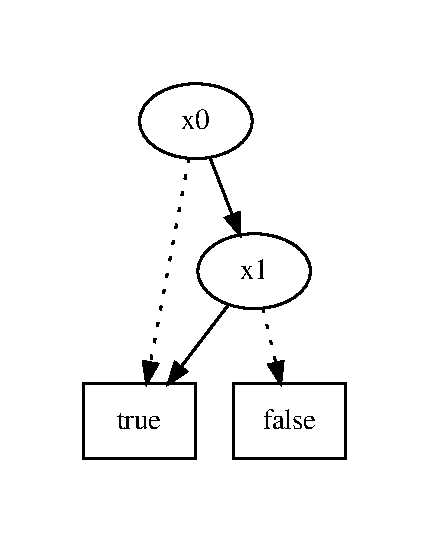
\includegraphics[trim = 0cm 1.5cm 0cm 1cm , scale=0.6]{exemple/impl_simple}
  \caption{ADB d'un implication simple : $x_0 \Rightarrow x_1$}
\end{figure}
Cet arbre se lit de haut en bas : on commence par évaluer la première variable, soit à $vrai$ soit à $faux$. Ensuite on arrive dans un autre état où la première variable n'existera plus et sera remplacé par son évaluation.\\
On réitère ensuite ce processus pour les variables qui suivent.\\
La flèche en pointillée représente le chemin à emprunter si la variable correspondant au nœud a 0 pour valeur de vérité et la flèche pleine correspond à la valeur de vérité 1.\\
Ici, on voit bien que si $x_0$ est faux, alors l'implication est vrai, quelque soit la valeur de vérité de $x_1$.\\
Si $x_0$ est vrai, alors il faut regarder la valeur de vérité de $x_1$ : si $x_1$ est vrai, alors l'implication est vraie et si $x_1$ est faux alors l'implication est fausse.\\

Ici, on a aussi introduit l'idée que cet arbre est ordonné, qu'on notera \textit{ADBO} (arbre de décision binaire ordonné).\\
Il faut donner un ordre aux variables pour savoir dans quel ordre on va attribuer une valeur de vérité aux variables pour former l'arbre.\\
On le présentera plus en détail plus tard, mais il s'avère que l'arbre dépend de l'ordre choisi : on peut obtenir un arbre plus petit avec un certain ordre et un autre beaucoup plus grand avec un autre ordre.\\

Enfin, introduisons la notion d'unicité de cet arbre. La construction de l'arbre est unique en fonction de l'ordre choisi, c'est à dire qu'en ayant fixé un ordre, toutes les expressions équivalentes posséderont le même ADB. On le notera \textit{ADBOC} (arbre de décision binaire ordonné canonique).\\
 
\section*{Organisation}
On va ici vous présenter les résultats de notre recherche sur le sujet.\\
Dans un premier temps, on va vous présenter les propriétés d'un ADBOC et la raison pour laquelle on peut générer pour toutes \expps un ADBOC.\\
Ensuite, nous présenterons l'algorithme que nous avons implémenté en Ocaml pour pouvoir générer ces ADBOCs. Nous discuterons aussi de la complexité de cet algorithme.\\
Enfin, nous présenterons les intérêts des ADBOCs ainsi que des réflexions qu'on peut avoir sur leurs utilisations.  



%%%%% Chapitre 1 %%%%%%%
\chapter{Représentation sous ROBDD}

\section{Système complet de $\varphi$}
\section{démo de l'existence}
\section{démo de l'unicité}
\section{A quoi correspond le graphe, et rapport avec $\varphi$}
\section{Représentation correcte -> pas de perte d'informations}

%%%%% Chapitre 2 %%%%%%%
\chapter{Construction d'une ROBDD}

On a implémenté tout un algorithme (en Ocaml) prenant en argument une expression propositionnelle et permettant d'obtenir l'ADBOC de celle-ci.\\
On va vous présenter les fonctions principales.

\section{présentation de l'algorithme}

Il faut déjà comprendre que l'algorithme implémenté est dans un paradigme impératif et qu'on va utiliser une structure correspondante à une Hashmap : l'accès à un élément est linéaire amorti et l'ajout est en temps linéaire amorti, c'est à dire qu'on peut faire ces opérations en temps constant dans un moyenne des temps mais en temps linéaire dans le pire des cas.\\
Notons avant de comprendre l'algorithme en détail que nous avons une structure, noté $S$, qui nous permet d'associer un nœud de l'arbre à ses deux nœuds enfants : on notera \textit{low} pour le nœud suivant la valuation à \textit{faux} et \textit{high} le nœud correspondant à la valuation \textit{vrai} de la variable du nœud parent.\\
Enfin, on indicera les variables par leur rang dans l'ordre : $x_n$ est la $n$-ième variable, $n\in \mathbb{N}$ et $n\geq 0$.\\

L'algorithme est basé sur un principe récursif, on refait la même étape jusqu'à atteindre la condition de fin :
\begin{enumerate}
\item \label{order_eval} On détermine l'ordre d'évaluation des variables en fonction de l'ordre donné, pour obtenir un arbre ordonné.
\item \label{start_eval} On évalue l'\expp donné en argument pour voir si la valuation n'est pas déjà déterminable. Par exemple, si on a $0 \wedge x$ avec $x$ une variable propositionnelle, alors on sait déjà que quelque soit la valuation de $x$, l'expression est fausse.
\item Si la valuation est déterminé, on renvoie la nœud de l'arbre correspondant à la valeur de vérité correspondante (\textit{vrai} ou \textit{faux}).
\item Sinon, on crée le nœud \textit{low} et le nœud \textit{high} : 
 \begin{itemize}
\item \textit{low} correspond au nœud créé quand on repasse par l'étape \ref{start_eval} où on a remplacé la variable évaluée par $0$ et où on évalue par la variable suivante dans l'ordre de l'étape \ref{order_eval}.
\item \textit{high} correspond au nœud créé quand on repasse par l'étape \ref{start_eval} où on a remplacé la variable évaluée par $1$ et où on évalue par la variable suivante dans l'ordre de l'étape \ref{order_eval}.
\end{itemize}
\item Ensuite, on regarde si le nœud avec comme suivant \textit{low} et \textit{high} n'a pas déjà été créé, auquel cas on le crée, sinon on récupère le nœud déjà créé. Cela permet d'être sur qu'on obtient bien un arbre canonique.
\item Enfin, on renvoie le nœud créé. A la fin de l'algorithme, le dernier nœud renvoyé correspondra à la racine de l'arbre.
\end{enumerate}

\section{Création d'un nœud}

On vous présente en simplifier le code de la fonction qui s'occupe de créer un nouveau nœud en cas de besoin. Ensuite nous commenterons les différentes lignes.
\begin{lstlisting}
let mk (i : indice de la variable) (low : noeud) (high : noeud) : node =
    if low = high then low      (* #1 *)
    else
    if member i low high then   (* #2 *)
      lookup i low high         (* #3 *)
    else
      create_node i low high    (* #4 *)
\end{lstlisting}
On regarde d'abord si on obtient le même résultat quelque soit la valuation de la i-ème variable ($\#1$). Si c'est le cas, on renvoie le nœud correspondant à une des deux valuations (on garde la canonicité).\\
Si ce n'est pas le cas, on regarde si on n'a pas déjà créé un nœud ayant le même \textit{low} et le même \textit{high} ($\#2$), auquel cas on renvoie ce nœud ($\#3$).\\
Enfin, si le nœud n'existe pas, alors on le crée ($\#4$).\\
Dans le meilleur des cas, la création se fait en temps constant et dans le pire des cas, elle se fait en temps linéaire (à cause de la Hashmap).

\section{Construction de l'arbre}

On va ensuite pouvoir exposer l'algorithme correspondant à la construction même de l'arbre.
\begin{lstlisting}
let build (f : exp propositionnelle) : noeud = 
    let tab = Array.init (!n) (function a -> None) in
    let rec aux (f : exp propositionnelle) (i : indice de la variable) : node =
      match getBool f tab with 									(* #1 *)
      | (None, nf) -> begin										(* #2 *)
          if i >= (!n) then failwith "exception de getBool"		(* #3 *)
          else begin
            let v0 = tab.(i) <- (Some false); aux nf (i+1) in	(* #4 *)
            let v1 = tab.(i) <- (Some true); aux nf (i+1) in	(* #5 *)
            tab.(i) <- None;	
            mk i v0 v1											(* #6 *)
          end
        end
      | (Some b, _) -> 											(* #7 *)
        if b then 1
        else 0
    in
    aux f 0
\end{lstlisting}
L'initialisation du tableau \textit{tab} correspond à l'évaluation partielle de chacune des variables.\\
Ensuite, on fait une fonction récursive qui se déroule en $7$ étapes :
\begin{enumerate}
\item On fait l'évaluation partielle de l'\expp pour voir si on ne peut pas déterminer sa valeur sans avoir donné une valuation à chaque variable ($\#1$).\\
\item Si ce n'est pas le cas ($\#2$), on vient effectuer le corps de l'algorithme en construisant de nouveaux nœuds. Ici, nous avons aussi effectué une optimisation de l'algorithme en faisant en sorte que, lors de l'évaluation partielle, on factorise l'\expp dans un même temps (correspond à la variable \textit{nf} dans $\#2$).
\item Si on se retrouve dans la situation où on a déjà donné une valeur de vérité à toutes les variables et qu'on est dans une situation indéterminée, alors on a une erreur d'algorithme ($\#3$).
\item Si on ne rencontre pas cette situation, on va récupérer le nœud correspondant à la valuation. Et donc on vient récupérer le nœud pour l'évaluation de la variable à $0$ ($\#4$), donc ce qui correspond au \textit{low}.
\item Ensuite, on récupère pour la valuation à $1$ ($\#5$).\\
\item Enfin, on récupère le nœud correspondant (création ou récupération d'un nœud déjà existant : dépend de la fonction \textit{mk}), et on renvoie ce nœud.
\item Si, par contre, on se retrouve à avoir une valuation déjà déterminée, alors on se retrouve dans la situation $\#7$, et la on renvoie le nœud correspond à \textit{vrai} ou à \textit{faux}.
\end{enumerate}
Notre algorithme suit la logique où on donne une valuation $1$ ou $0$ à chaque variable, et donc on aurait une complexité de $2^n$ à chaque fois. Cependant, il fait cela de façon intelligente, et on ne se retrouve pas deux fois dans une même situation. On peut dire que c'est une sorte d'algorithme dynamique (à l'aide des hashmap).\\

\section{Sat-solveur}
On a ensuite défini des fonctions de parcours de cette arbre et qui nous permettent d'obtenir des informations intéressantes avec notre arbre déjà construit.

\subsection{SatCount}
La première fonction est une fonction en temps linéaire du nombre de nœud de notre arbre et qui permet de déterminer combien est ce qu'il y a de valeurs de vérité qui satisfassent une \expp.
\begin{lstlisting}
let satCount (u : noeud) : int =
    let node_of_var = ... in									(* #1 *)
    let rec aux (u : noeud) : (distance au noeud true, nombre de possibilites)  = 
      if u = 0 then (0,0) 			
      else if u = 1 then (0,1) 									(* #2 *)
      else
        let ind = node_of_var.(u) in
        let som = 
          let (i,res) = aux (low u) in two_power (ind - i - 1) * res (* #3 *)
                        +
          let (i, res) = aux (high u) in two_power (ind - i - 1) * res
        in (ind, som)
    in
	let size = Array.length !var_tab in
    if u = 0 then 0												(* #4 *)
    else if u = 1 then two_power size							(* #5 *)
    else let (i,res) = aux u in two_power (size - i) * res	(* #6 *)
\end{lstlisting}

Pour pouvoir compter le nombre de valeurs de vérité possible, on a besoin de savoir à quelle variable correspond chaque nœud (plus précisément, on renvoie l'indice de la variable et qui commence à $1$). C'est dans ce but là qu'on initialise le tableau \textit{node\_of\_var} ($\#1$).\\
Ensuite, on va faire une fonction récursive locale à la fonction \textit{aux} : elle prend un nœud de l'arbre en argument et renvoie un couple contenant la distance du nœud à \textit{true} et le nombre de valuation possible depuis ce nœud là.\\
Si on tombe sur le nœud \textit{vrai}, on renvoie le couple $(0,1)$, car la distance à lui-même est à $0$ et on a une solution possible, et $(0,0)$ pour \textit{faux} ($\#2$).\\
Ensuite, si on n'est pas sur une constante, on calcule pour chaque valuation de la variable combien on a de solutions possibles ($\#3$) :

\begin{itemize}
\item On récupère le couple de \textit{low} et de \textit{high}.
\item Si la variable suivante (\textit{low} ou \textit{high}) possède un indice dont la différence est supérieure à $1$, alors lors de la construction, on s'est retrouvé à faire une simplification du nœud parce qu'il amenait à la même valeur de vérité. Donc le nombre de solutions correspond à $2^{difference~des~distances~-~1}$.
\end{itemize}
Lorsqu'on sort de la boucle, il ne nous reste plus qu'à multiplier le nombre de solution de la racine par $2^{distance~avec~le~nombre~de~variables}$.\\
On obtient ainsi le nombre de solutions possibles.

\subsubsection{AnySat}

Lorsque la construction de l'arbre a été effectué, on peut déterminer en tant constant si une \expp est une antilogie (s'il n'y a qu'un seul nœud et qu'il correspond à \textit{faux}). De plus, on peut trouver, en temps linéaire du nombre de variables, une valuation satisfaisant notre \expp.

\begin{lstlisting}
let rec anySat (u : noeud) : (variable * bool) list =
    let rec aux u = 
      if u = 0 then raise (No_SAT "Solution introuvable")
      else if u = 1 then []
      else if low u = 0 then (!var_tab.(var u), true) :: (aux (high u))
      else (!var_tab.(var u), false) :: (aux (low u))
    in
    fill_var 0 (aux u)
\end{lstlisting}
Il suffit de parcourir notre nœud racine et d'arriver jusqu'au nœud \textit{vrai}. Pour cela, on a choisi de passer par \textit{low}, mais on aurait très bien pu passé par \textit{high}, car si \textit{low} et \textit{high} existe et sont différents de \textit{faux}, alors il y a un chemin permettant d'aller à \textit{vrai}.\\
On est en temps linéaire du nombre de variable car à chaque itération, on descend d'un cran vers \textit{vrai}, et donc on donne une valuation à chaque variable.\\
La dernière opération, appelé \textit{fill\_var}, permet de remplir la solution en attribuant une valeur de vérité à toutes les variables dont un nœud correspondant n'a pas été visité. Cela permet d'obtenir une solution attribuant une valeur de vérité à chaque variable.

\subsubsection{AllSat}

De la même façon, on peut aussi obtenir l'ensemble des solutions possibles en temps linéaire selon le nombre de nœud de l'arbre :
\begin{lstlisting}
let allSat (u : node) : (variable * bool) list list =
    let rec aux (u : noeud) l r =
      if u = 0 then r
      else if u = 1 then l::r
      else aux (high u) ((!var_tab.(var u), true)::l) (aux (low u) ((!var_tab.(var u), false)::l) r)
    in 
    List.rev (List.rev_map (fun a -> fill_var 0 a) (aux u [] []))
\end{lstlisting}
Ici, à chaque nœud, on a comme argument l'ensemble des solutions possibles pour les nœuds parents. Ensuite, on teste si on arrive à \textit{vrai} en évaluant la variable, et si c'est possible, on ajoute la valuation à l'ensemble des valuations possibles.\\
On se retrouve ainsi à obtenir l'ensemble des solutions possibles en temps linéaire selon le nombre de nœud.\\

On vous a beaucoup parlé de l'algorithme, mais maintenant passons à la pratique.

\section{exemple d'exécution de l'algo}
\section{Etude des complexités}

%%%%% Chapitre 3 %%%%%%%
\chapter{Intérêt et optimisation}

\section{Raison de la ROBDD}
\section{Utilisation possible comme Sat-solveur mais mauvais}
\section{Théorie sur les ordres}

%%%%% Conclusion %%%%%%%
\chapter*{Conclusion}
\addcontentsline{toc}{chapter}{Conclusion}

\section*{Nouvelle approche d'une expression propositionnelle}
\section*{Optimisation que cela apporte en fonction de l'ordre}
\section*{Représentation simple d'une expression prop}
\section*{Théorie développée et approche de recherche pour les ordres}
\section*{Ce que le projet nous a apporté}

%%%%% Bibliographie %%%%%%%
\chapter*{Bibliographie}
\addcontentsline{toc}{chapter}{Bibliographie}
Ajouter les différents articles sur lesquels on s'est basé.

\end{document}